\documentclass[tikz,border=8pt]{standalone}
\usepackage[T1]{fontenc}
\usepackage{lmodern}
\usepackage{amsmath}

\begin{document}
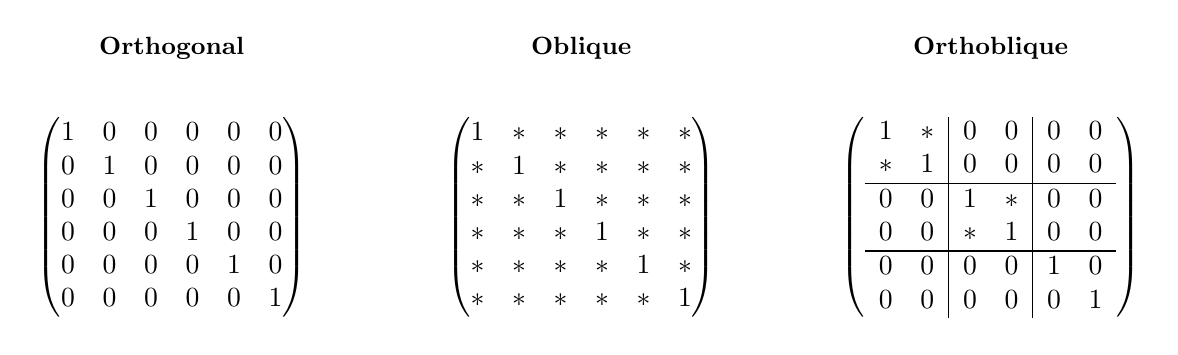
\begin{tikzpicture}

% Titles
\node[font=\small\bfseries] at (0,2.15) {Orthogonal};
\node[font=\small\bfseries] at (5.2,2.15) {Oblique};
\node[font=\small\bfseries] at (10.4,2.15) {Orthoblique};

% Orthogonal: six mutually orthogonal factors
\node at (0,0) {$\begin{pmatrix}
1&0&0&0&0&0\\
0&1&0&0&0&0\\
0&0&1&0&0&0\\
0&0&0&1&0&0\\
0&0&0&0&1&0\\
0&0&0&0&0&1
\end{pmatrix}$};

% Oblique: all correlations free
\node at (5.2,0) {$\begin{pmatrix}
1&\ast&\ast&\ast&\ast&\ast\\
\ast&1&\ast&\ast&\ast&\ast\\
\ast&\ast&1&\ast&\ast&\ast\\
\ast&\ast&\ast&1&\ast&\ast\\
\ast&\ast&\ast&\ast&1&\ast\\
\ast&\ast&\ast&\ast&\ast&1
\end{pmatrix}$};

% Orthoblique: two oblique blocks and two orthogonal factors
\node at (10.4,0) {$\left(
\begin{array}{cc|cc|cc}
1&\ast&0&0&0&0\\
\ast&1&0&0&0&0\\ \hline
0&0&1&\ast&0&0\\
0&0&\ast&1&0&0\\ \hline
0&0&0&0&1&0\\
0&0&0&0&0&1
\end{array}
\right)$};

\end{tikzpicture}
\end{document}